\documentclass[
	openany,
	% -- opções da classe memoir --
	12pt,				% tamanho da fonte
   % openright,
	%twoside,
    oneside,
    % para impressão em verso e anverso. Oposto a oneside
	a4paper,			% tamanho do papel. 
	brazil				% o último idioma é o principal do documento
	]{abntex2}

% ---
% Pacotes básicos 
% ---

\usepackage{fontspec}
\setmainfont{Arial}

\usepackage[utf8]{inputenc}		% Codificacao do documento (conversão automática dos acentos)
\usepackage{indentfirst}		% Indenta o primeiro parágrafo de cada seção.
\usepackage{color}				% Controle das cores
\usepackage{graphicx}			% Inclusão de gráficos
\usepackage{microtype} 			% para melhorias de justificação
\usepackage{multicol}			% multiplas colunas no texto
\usepackage{subcaption}
\usepackage{caption}
\usepackage{float}
\usepackage{amsmath}
\usepackage{amssymb}
\usepackage{amsthm}
\usepackage{lipsum}
\usepackage{blindtext}
\usepackage{lscape}
\usepackage{booktabs}
\usepackage{hyperref}

%\usepackage[square,sort&compress,comma,numbers,nonamebreak,longnamesfirst]{natbib}

% ---
% ---
% Pacotes de citações
% ---
\usepackage[brazilian]{backref}	 % Paginas com as citações na bibl
\usepackage[alf]{abntex2cite}	% Citações padrão ABNT

% --- 
% CONFIGURAÇÕES DE PACOTES
% --- 

% ---
% Configurações do pacote backref
% Usado sem a opção hyperpageref de backref
\renewcommand{\backrefpagesname}{Citado na(s) página(s):~}
% Texto padrão antes do número das páginas
\renewcommand{\backref}{}
% Define os textos da citação
\renewcommand*{\backrefalt}[4]{
	\ifcase #1 %
		Nenhuma citação no texto.%
	\or
		Citado na página #2.%
	\else
		Citado #1 vezes nas páginas #2.%
	\fi}%
% ---

% ---
% Informações de dados para CAPA e FOLHA DE ROSTO
% ---
\titulo{Modelos Computacionais para a Simulação e Análise da Detecção de Ondas Gravitacionais.}
\autor{Gerson Rodrigues Santos}
\local{Recife}
\data{2018}
\orientador{Prof. Tiago A. E. Ferreira}
\coorientador{Prof. Antônio de Pádua Santos}


\instituicao{%
	Universidade Federal Rural de Pernambuco -- UFRPE
  	\par
  	Departamento de Estatística e Informática
    \par
  	Mestrado em Informática Aplicada
}

\tipotrabalho{Trabalho de Conclusão de Curso}
% O preambulo deve conter o tipo do trabalho, o objetivo, 
% o nome da instituição e a área de concentração 
\preambulo{Projeto de Dissertação apresentado ao Curso de Mestrado em Informática Aplicada da Universidade Federal Rural de Pernambuco como requisito parcial para conclusão do Curso.}
% ---


% ---
% Configurações de aparência do PDF final

% alterando o aspecto da cor azul
\definecolor{blue}{RGB}{41,5,195}

% informações do PDF
\makeatletter
\hypersetup{
     	%pagebackref=true,
		pdftitle={\@title}, 
		pdfauthor={\@author},
    	pdfsubject={\imprimirpreambulo},
	    pdfcreator={LaTeX with abnTeX2},
		colorlinks=true,       		% false: boxed links; true: colored links
    	linkcolor=blue,          	% color of internal links
    	citecolor=blue,        		% color of links to bibliography
    	filecolor=magenta,      		% color of file links
		urlcolor=blue,
		bookmarksdepth=4
}
\makeatother
% --- 

% --- 
% Espaçamentos entre linhas e parágrafos 
% --- 

% O tamanho do parágrafo é dado por:
\setlength{\parindent}{1.3cm}

% Controle do espaçamento entre um parágrafo e outro:
\setlength{\parskip}{0.2cm}  % tente também \onelineskip

% ---
% compila o indice
% ---
\makeindex
% ---

% ----
% Início do documento
% ----
\begin{document}

% Seleciona o idioma do documento (conforme pacotes do babel)
%\selectlanguage{english}
\selectlanguage{brazil}

% Retira espaço extra obsoleto entre as frases.
\frenchspacing 

% ----------------------------------------------------------
% ELEMENTOS PRÉ-TEXTUAIS
% ----------------------------------------------------------
% \pretextual
%\begin{figure}[h]
%\centering % este comando é usado para centralizar a figura
%
\includegraphics[width=7cm]{figuras/logo_ufrpe_horizontal.png}\\
%\end{figure}

% \begin{figure}[ht]
% \centering
% \begin{minipage}[b]{0.45\textwidth}
% 
\includegraphics[height=3cm]{figuras/logo_ufrpe_horizontal.png}
% \end{minipage}
% \qquad
% \begin{minipage}[b]{0.45\textwidth}
% \includegraphics[height=2.5cm]{figuras/logo_bsi.pdf}
% \end{minipage}
% \end{figure}

%\begin{minipage}[t]{1\textwidth}
	\begin{figure}[ht]
		
\includegraphics[height=4cm]{figuras/logo_ppgia.png}
	\end{figure}
%\end{minipage}

% ---
% Capa
% ---
\imprimircapa
% ---
% ---
% Folha de rosto
% (o * indica que haverá a ficha bibliográfica)
% ---
\imprimirfolhaderosto
% ---

% dedicatoria
\begin{dedicatoria}
   \vspace*{\fill}
   \centering
   \noindent
   \textit{À \ldots\\} \vspace*{\fill}
\end{dedicatoria}

% agradecimentos
\begin{agradecimentos}
Agradeço à \ldots

\end{agradecimentos}

% epigrafe
\begin{epigrafe}
    \vspace*{\fill}
	\begin{flushright}
		\textit{``A Ciência não tem medo de assumir a sua ignorância, de assumir os limites do que podemos explicar e com isso avançar. Quem se contenta com explicações fechadas e definitivas, ficam com elas. Nós, ficamos com eventos cósmicos capazes de mudar o universo.'' \\
		(Albert Einstein)}
	\end{flushright}
\end{epigrafe}

% resumo e abstract
\setlength{\absparsep}{18pt} % ajusta o espaçamento dos parágrafos do resumo
\begin{resumo}
 
\lipsum[1]

 \textbf{Palavras-chave}: palavra 1, palavra 2, \ldots.
\end{resumo}


\begin{resumo}[Abstract]
 \begin{otherlanguage*}{english}
  
  \lipsum[1] 

   \vspace{\onelineskip}
 
   \noindent 
   \textbf{Keywords}:  word 1, word 2, \ldots.
 \end{otherlanguage*}
\end{resumo}

% ---
% inserir lista de ilustrações
% ---
\pdfbookmark[0]{\listfigurename}{lof}
\listoffigures
\cleardoublepage
% ---

% ---
% inserir lista de tabelas
% ---
\pdfbookmark[0]{\listtablename}{lot}
\listoftables*
\cleardoublepage
% ---

% ---
% inserir lista de abreviaturas e siglas
% ---
\begin{siglas}
  \item[UDP] User Datagram Protocol	
  \item[TCP] Transmission Control Protocol
  \item[...] \ldots
\end{siglas}
% ---

% ---
% inserir o sumario
% ---
\pdfbookmark[0]{\contentsname}{toc}
\tableofcontents*
\cleardoublepage
% ---



% ----------------------------------------------------------
% ELEMENTOS TEXTUAIS
% ----------------------------------------------------------
\textual

% ----------------------------------------------------------
% inclusao das secoes do texto
% ----------------------------------------------------------
\chapter{Introdução}
A maneira que temos de observar a natureza e o universo sempre dependeu de instrumentos, microscópios trouxeram a noção de que micro-organismos extremamente pequenos existiam, nos permitiram descobrir as bactérias, as formas de vida mais comuns do planeta, telescópios nos deram habilidades de observar o sistema solar descobrir as órbitas dos planetas e formular a noção de gravidade de Newton \cite{newton1687philosophiae}. 

Mas nem sempre essas descobertas aconteceram de propósito. Em 1930, o físico Karl Jansky foi encarregado de melhorar os sinais de rádio que cruzavam os oceanos com telégrafos e chamadas de telefone, para detectar de onde vinham as ondas de rádio que atrapalhavam a chamada com estática. Jansky construiu uma antena giratória que podia apontar para todas as direções. Foi quando ele descobriu ondas de rádio vindas de tempestades de raios próximas e distantes e uma terceira fonte de rádio no céu. O sinal ficava mais forte a cada 23 horas e 56 minutos, o tempo que as estrelas levam para percorrer o céu, o nosso dia sideral \cite{singh2010big}. 

O ponto que ele descobriu, era o centro da nossa Via Láctea, com a maior parte dos sinais de rádio vindos da constelação de sagitário. De alguma forma o universo estava cheio de fontes de ondas de rádio, uma descoberta por acaso, feita sem querer por alguém que estava preparado para entender o que havia encontrado, uma serendipidade. 
Assim como o sol emite radiação eletromagnética na forma de ondas de luz. Também emite frequências maior e menor, como rádio. Com apenas 26 anos, Jansky publicou o trabalho que inaugurou a radioastronomia, a observação do universo com os radiotelescópios, que nos permite ver, de explosões aos bips de pulsares \cite{jansky1932directional}. Como ver em outras ondas além da luz nos mostra novos fenômenos, observações de raio-x, por exemplo, mostram buracos negros rasgando as estrelas \cite{200814}, os quasares, em quanto a radiação infravermelha atravessa a Via Láctea e nos mostra o que tem por trás dela. 

E o que a descoberta da radioastronomia teve de serendipidade, a descoberta das ondas gravitacionais (Gravitational wave) (GW) teve de proposital. Começando por Einstein. Em 1915, quando ele adicionou a gravidade à teoria da relatividade, Publicando a "Teoria da Relatividade Geral" \cite{albert1920realtivity}, Einstein concluiu que a gravidade não era uma força, mas sim a deformação do espaço tempo, e essa deformação do espaço deveria viajar pelo universo como uma onda, viajando na velocidade da luz, mas isso só havia sido observado indiretamente. 

Por volta de 1960, descobertas astronômicas (quasares, pulsares, radiação cósmica de fundo) e novos experimentos impulsionaram a relatividade geral, para a linha de frente. Neste período foi descoberto a diminuição no período orbital do pulsar binário Hulse-Taylor em uma taxa consistente com a predição da relatividade geral da perda de energia por ondas gravitacionais \cite{weisberg2004relativistic}, e essa havia sido a primeira detecção indireta de ondas gravitacionais da historia da ciência, havia, por que agora, observamos pela primeira vez, dois buracos negros se fundindo e liberando uma energia 10 vezes maior do que a emissão de luz por todas as galáxias do universo observável. 

Pra isso precisamos do Observatório de Ondas Gravitacionais por Interferometria a Laser (Advanced Laser Interferometer Gravitational Wave Observatory) (aLIGO) \cite{PhysRevLett.116.131103,0264-9381-32-7-074001}, que recentemente, até o momento, tem anunciado a detecção de ondas gravitacionais a partir de medidas de uma série de eventos cósmicos que envolvem colapso de sistemas binários formados por objetos compactos tais como buracos negros \cite{abbott2016observation,ligo2016gw151226,scientific2017gw170104,abbott2017gw170814}, e estrelas de nêutrons \cite{abbott2017gw170817}, que são consistentes com as previsões gerais de relatividade de Einstein.

O observatório tem dois centros, com formato em L um posicionado em Washington e outro em Louisiana nos Estados Unidos, na quina desse L um espelho divide um feixe de laser em duas partes, que percorrem, cada uma, um dos tubos de 4 kilômetros e encontra um espelho lá no final, quando as ondas de laser voltam, se anulam e desaparecem se um dos tubos for deslocado por causa de uma deformação do espaço e do tempo, muda a distância percorrida pelo laser, e o sinal deixa de ser cancelado, como ilustra a Figura~\ref{figinterferometer}, pra garantir que a deformação foi causada por uma onda gravitacional e não um terremoto ou outro problema, o mesmo sinal tem que ser observado nos dois centros \cite{PhysRevLett.116.131103}. 

\begin{figure}[ht]
\centering
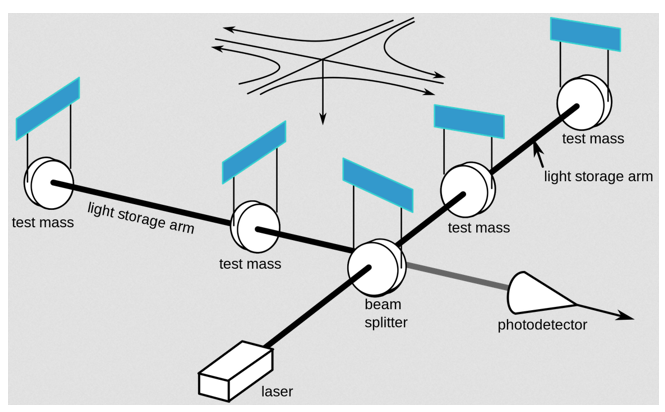
\includegraphics[width=1\textwidth]{figuras/interferometro.png}
\caption{Diagrama de um projeto básico de interferômetro. [Image: LIGO]}
\label{figinterferometer}
\end{figure}
 
Após a parada do LIGO nos periodos de 2010 à 2015 o observatorio foi parado para passar por um upgrade na capacidade de detecção e logo no inicio de suas atividade ele captou o primeiro sinal de uma colisão de buracos negros, há 1,3 bilhão de anos luz daqui, que levando ao prêmio Nobel de Física em 2017 \cite{abbott2016observation}. 
 
Quando um objeto denso e massivo é acelerado, ele cria ondas gravitacionais como as ondas que uma pedra lançada em um lago produz, e de acordo com Einstein, nada é mais denso e massivo do que um buraco negro. E o sistema binário, dois buracos negros giram um ao redor do outro, na primeira detecção que foi observada \cite{abbott2016observation}, um deles tinha a massa de 36 sóis e o outro de 29 conforme eles giram em órbita, emitem ondas gravitacionais e com isso perdem energia, conforme perdem energia, se aproximam ainda mais e giram ainda mais rápido quanto mais se aproximam, mais energia perdem e mais ondas emitem e mais se aproximam cada vez mais rápido até colidirem.

No final da explosão o buraco resultante ficou com 62 massas solares, os 3 sóis de diferença foram convertidos em ondas gravitacionais, conforme os buracos negros se aceleram antes da colisão, as ondas que emitem ficam cada vez mais intensas e cada vez mais frequentes, até virarem um gorjeio, que marca a colisão, um gorjeio emitido há mais de 1 bilhão de anos, uma explosão tão forte, que chacoalhou o espaço e o tempo e conseguimos captar daqui.

Agora temos a confirmação de que as ondas gravitacionais previstas há 100 anos existem, e sabemos como detectá-las. Em pouco tempo teremos detectores como LIGO em órbita da terra, com sensores há milhares de quilômetros de distância, capazes de detectar ondas gravitacionais ainda menores. Agora podemos captar as ondas emitidas pela explosão de supernovas ou pela fusão de estrelas de nêutrons formando buracos negros.


\section{Delimitação do Tema}

A natureza nem sempre pode ser observada em sua plenitude, mas sempre poderá ser simulada computacionalmente desde que existam os apropriados modelos computacionais. Neste sentido, a computação científica e numérica desempenha o papel de ferramenta fundamental da área da ciência da computação para o entendimento da natureza, explicitando fenômenos e dinâmicas muitas vezes não possíveis de serem observados pela limitada capacidade humana de observação.

Em particular, para a geração de modelos computacionais que venham a descrever a gravidade é necessário entender como o universo funciona. A teoria da Relatividade de Einstein \cite{albert1920realtivity} mostra que o espaço e o tempo não são entidades separadas. Desta forma, o espaço e o tempo formam um contínuum conhecido como espaço-tempo que participa da dinâmica dos eventos. As equações da Relatividade Geral de Einstein mostram que a dinâmica da matéria está conectada à curvatura do espaço-tempo. A gravidade é, portanto, uma manifestação da curvatura do espaço-tempo.

Um dos aspectos da dinâmica do espaço-tempo é radiação gravitacional. Prevista pela Teoria da Relatividade Geral em 1916, a descoberta das ondas gravitacionais tem sido um objetivo perseguido por cerca de 100 anos. A descoberta das ondas gravitacionais seria mais uma confirmação da Teoria da Relatividade Geral que se somaria às outras confirmações das Teoria de Einstein, tais como a deflexão da luz ao passar com objetos massivos como estrelas, lentes gravitacionais, a explicação do desvio do periélio do planeta Mercúrio, efeitos relativísticos nas órbirtas dos planetas, buracos negros, etc. 

Os efeitos Relativísticos de natureza gravitacionais são de grande importância à atual tecnologia e com aplicação à vida diária das pessoas. Um dos principais resultados da Teoria da Relatividade Geral foi a possibilidade de permitir a localização de coordenadas na superfície de planetas com extrema precisão (o equivalente ao georreferenciamento, contudo extraterrestre, a partir da Terra). A localização de coordenadas na superfície de planetas é uma das aplicações tecnológicas que só foi possível com uso da Teoria da Relatividade Geral. O resultado de tal tecnologia aplicado ao caso do planeta Terra foi o desenvolvimento da tecnologia do Sistema de Posicionamento Global GPS (Global Positioning System).

Por outro lado, a busca da detecção de ondas gravitacionais continua intensa, a análise e o tratamento computacional destas informações encontram-se na crisa da onda da tecnologia computacional para o entendimento de tal processo.

\section{Problema de Pesquisa}
Para que seja possível a detecção de GW é necessário um grande esforço contínuo dos detectores de GW e das instalações astronômicas e a natureza sensível a tempo dessas análises requer algoritmos que podem detectar e caracterizar eventos GW em tempo real e o custo computacional das buscas de filtros combinados aumenta significativamente quando se direciona as fontes de GW que abrangem um espaço de parâmetro dimensional mais alto.

A filtragem combinada, o algoritmo de detecção de GW mais sensível usado pelo LIGO, atualmente tem como alvo fontes binárias compactas com componentes alinhados à rotação em órbitas quase circulares.  Estudos recentes também indicam que essas buscas podem perder GWs geradas por populações binárias compactas formadas em ambientes estelares densos. Estender essas buscas com correspondência de modelos para direcionar BBHs de precessão por rotação, quase-circulares ou excêntricas é proibitivamente computacional \cite{george2018deep}.

Acelerar os algoritmos de estimação de parâmetros bayesianos offline, que normalmente duram de várias horas a alguns dias, não é uma tarefa trivial. a resposta para esses desafios tem sido o esforço continuo para reduzir o tamanho dos bancos de modelos usados para pesquisas GW baseadas em filtragem combinada \cite{indik2017reducing}. Com base nessas considerações, e percebendo que, para maximizar a ciência que se pode extrair das observações de GW, é essencial cobrir rapidamente um espaço de parâmetro mais profundo de fontes de motivação astrofísica, a comunidade da GW vem explorando instalações de computação de alto desempenho (HPC) de última geração para aumentar o conjunto de recursos computacionais para realizar a análise de dados GW em larga escala \cite{huerta2017boss,weitzel2017data}.


\section{Objetivos}
A seguir serão apresentados os objetivos geral (OG) e específicos (OE) que nortearão a condução desta pesquisa.

\subsection{Objetivo Geral}
A presente pesquisa tem como objetivo geral o desenvolvimento de procedimentos computacionais baseados em computação científica e numérica para o entendimento da dinâmica gravitacional do universo, contribuindo para uma nova área de pesquisa computacional designada de Astroinformatics com o desenvolvimento de bibliotecas computacionais para análise estatística dos resultados experimentais reais de medida das ondas gravitacionais. Para atingir esse objetivo geral foram propostos os objetivos específicos a seguir relacionados.
\subsection{Objetivos Especificos}
Para atingir o objetivo geral foram definidos os seguintes objetivos específicos: 
\begin{itemize}

\item Estudo introdutório dos processos de modelagem matemática para a geração das equações que governam as ondas gravitacionais;
\item Estudo das metodologias computacionais para a resolução de sistemas de equações diferenciais parciais acopladas;
\item E Desenvolvimento e implementação de bibliotecas numéricas para a solução de sistemas de equações diferenciais parciais em uma plataforma de GP/GPU (CUDA);
\item Simulações computacionais de ondas gravitacionais em uma plataforma baseada em GP/CPU (CUDA);
\item Estudo de inferência estatística e análise de ruídos para verificação de aderência entre os resultados obtidos pelo LIGO e as soluções numéricas obtidas.

\end{itemize}
\section{Justificativa}

Com base em todas as considerações descritas, precisamos de um novo paradigma para superar as limitações e os desafios computacionais dos algoritmos de detecção de GW existentes. Um candidato ideal seria a inteligencia artificial, mais especificamente as Machine Learning, a qual hoje é tendencia no mercado, que é uma area  altamente escalável que pode aprender diretamente a partir de dados brutos, sem qualquer recurso manual de engenharia, usando camadas hierárquicas profundas de “neurônios artificiais”. redes, em combinação com técnicas de otimização baseadas em retro-propagação e gradiente descendente \cite{barca2005treinamento}. A Machine Learning, especialmente com o auxílio da computação GPU, alcançou recentemente um imenso sucesso em aplicações comerciais e em inteligência artificial \cite{esteva2017dermatologist}, \cite{moravvcik2017deepstack}, \cite{van2016wavenet}, \cite{10.1007/978-3-319-44188-7_16}, e também tem sido aplicado em astrofísica \cite{george2017glitch}, \cite{george2017deepA}.
\chapter{Revisão da Literatura}
Definição dos principais conceitos e categorias a serem utilizadas na pesquisa. A definição da base teórica e conceitual é um momento fundamental, pois proporciona a sustentação da pesquisa científica. Este capítulo 2 como um todo deve começar numa página nova e costuma ter entre 5 e 10 páginas.
Aqui você deverá apresentar os principais conceitos associados ao tema que está sendo investigado. É interessante subdividir (2.1, 2.2, 2.n) de acordo com seus temas de pesquisa. Os subtópicos das referências conceituais também guardam relação com o problema de pesquisa. Você só deve falar de conceitos que tem relação com seu problema. Aqui você deve mostrar a contribuição dos diversos autores que falam sobre o assunto que você está investigando, então é necessário citá-los. 
Muito cuidado neste momento para não incorrer em plágio, que é a apropriação indevida de textos produzidos por outros autores sem a devida citação conforme norma. Outro cuidado é para que o texto não fique parecendo uma colcha de retalhos, com as diversas partes sem nenhuma conexão. Procure encadear bem o texto.
\chapter{Metodologia}
Este capítulo objetiva definir a metodologia que será utilizada na pesquisa, bem como apontar quais ferramentas serão usadas na
condução, coleta de dados e análise dos dados.  
\section{Caracterização do Estudo}
A metodologia se refere ao caminho escolhido para se chegar ao fim proposto pela pesquisa. É a escolha que o pesquisador realizou para abordar o objeto de estudo e esta relacionada a relativamente seus elementos essenciais como (natureza, objetivos, procedimentos e abordagens)\cite{de2013metodologia}.

Este tópico tem por objetivo descrever os procedimentos e métodos científicos disponíveis para o desenvolvimento de uma pesquisa, bem como identificar o que melhor se enquadra às necessidades deste trabalho e permitir a reprodução deste trabalho por outros pesquisadores.

\subsection{Do ponto de vista da sua natureza}
No que diz respeito a sua natureza, ou seja, o tipo de contribuição que o estudo trará para a ciência, a pesquisa científica pode ser classificada em: pesquisa básica e pesquisa aplicada.

\textbf{a) pesquisa básica:} objetiva gerar conhecimentos novos úteis para o avanço da ciência sem aplicação prática prevista. Envolve verdades e interesses universais;

\textbf{b) pesquisa aplicada:} objetiva gerar conhecimentos para aplicação prática dirigidos à solução de problemas específicos. Envolve verdades e interesses locais.

\subsection{Do ponto de vista de seus objetivos}

A natureza de uma pesquisa está relacionada com seus objetivos gerais, sendo classicamente rotulada como exploratórias, descritivas ou explicativas \cite{gil2002elaborar}.

\textbf{a) Pesquisa exploratória:} esta pesquisa busca constatar algo em um determinado fenômeno de maneira a se familiar com o fenômeno investigado de modo que o próximo passo da pesquisa possa ser a construção de hipóteses.

\textbf{b) Pesquisa descritiva:} as pequisas descritivas tem como objetivo retratar as características do objeto estudado, expondo com precisão os fatos ou fenômenos, para estabelecer a natureza das relações entre as variáveis delimitadas no tema.

\textbf{c) Pesquisa explicativa:} essas pesquisas visam identificar os fundamentos que dão ensejo a um fenômeno, quer dizer, buscar a razão causa e o porquê das coisas. 

\subsection{Do ponto de vista dos procedimentos técnicos}
O delineamento da pesquisa é o que expressa em linhas gerais o desenvolvimento da pesquisa, ou seja, a maneira pela qual obtemos os dados necessários para a elaboração da pesquisa, e são definidos em dois grandes grupos de delineamentos: aqueles que se valem das chamadas fontes de papel (pesquisa bibliográfica e pesquisa documental) e aqueles cujos dados são fornecidos por pessoas (pesquisa experimental, pesquisa ex-post-facto, o levantamento, o estudo de caso, a pesquisa-ação e a pesquisa participante)\cite{de2013metodologia, gil2002elaborar}.

\textbf{a) Pesquisa bibliográfica:} Consiste na coleta de informações a partir de textos, livros, artigos e demais materiais de caráter científico, com o objetivo de colocar o pesquisador em contato direto com todo material já escrito sobre o assunto da pesquisa.

\textbf{b) Pesquisa documental:} a pesquisa documental, devido a suas características, pode ser confundida com a pesquisa bibliográfica, similar à pesquisa bibliográfica, a documental não se restringe apenas a coleta de informações de caráter científico. Na pesquisa documental qualquer documento com conteúdo informacional útil para a pesquisa pode ser usado, como jornais, revistas, catálogos, fotografias, atas, etc.

\textbf{c) Estudo de caso:} Ao contrário da pesquisa documental e bibliográfica, esse procedimento é empírico. Isso significa que não se restringe apenas ao levantamento de informações teóricas, mas também de observações e experiências, investigando a fundo sobre algum aspecto específico de determinado tema (indivíduo, fenômeno, ambiente, etc). 

\textbf{d) Pesquisa experimental:} a pesquisa experimental consiste em determinar um objeto de estudo, selecionar as variáveis que seriam capazes de influenciá-lo, definir as formas de controle e de observação dos efeitos que a variável produz no objeto.

\textbf{e) Levantamento (survey):} nesse tipo de pesquisa ocorre quando envolve a interrogação direta das pessoas cujo comportamento / interação desejamos conhecer.

\textbf{f) Pesquisa de campo:} pesquisa de campo é aquela utilizada com o objetivo de conseguir informações e/ou conhecimentos acerca de um problema para o qual procuramos uma resposta, ou de uma hipótese, que queiramos comprovar, ou, ainda, descobrir novos fenômenos ou as relações entre eles.

\textbf{g) Pesquisa ex-post-facto:} quando o “experimento” se realiza depois dos fatos. A pesquisa ex-post-facto analisa situações que se desenvolveram naturalmente após algum acontecimento. É muito utilizada nas ciências sociais, pois permite a investigação de determinantes econômicos e sociais do comportamento da sociedade em geral. Estudamos um fenômeno já ocorrido, tentamos explicá-lo e entendê-lo.

\textbf{h) Pesquisa-ação:} quando concebida e realizada em estreita associação com uma ação ou com a resolução de um problema coletivo. Os pesquisadores e os participantes representativos da situação ou do problema estão envolvidos de modo cooperativo ou participativo.

\textbf{i) Pesquisa participante:} quando se desenvolve a partir da interação entre pesquisadores e membros das situações investigadas.

\subsection{Do ponto de vista da forma de abordagem do problema}

Do ponto de vista da abordagem usada pelo pesquisador no estudo, este pode ser categorizado em: pesquisa qualitativa ou quantitativa\cite{de2013metodologia}.

\textbf{a) Pesquisa quantitativa:} considera que tudo pode ser quantificável, o que significa traduzir em números opiniões e informações para classificá-las e analisá-las. Esse tipo de metodologia é caracterizado por usar técnicas e ferramentas estatísticas como principal meio de análise dos dados obtidos em uma pesquisa. 

\textbf{b) Pesquisa qualitativa:} considera que há uma relação dinâmica entre o mundo real e o sujeito, isto é, um vínculo indissociável entre o mundo objetivo e a subjetividade do sujeito que não pode ser traduzido em números. Se caracteriza por atribuir interpretações de natureza subjetiva. 

Analisando-se os conceitos e as considerações anteriormente descritas sobre a metodologia de pesquisa, mostra-se como mais adequado para a presente pesquisa a de natureza básica, de caráter descritivos, que partem de procedimentos técnicos experimentais, de cunho qualitativo, sendo estes mais apropriados aos objetivos desta pesquisa.
\section{Coleta de Dados}
Tanto para o processo de treinamento quanto para o processo de teste de uma RNA, o primeiro passo a ser dado é a obtenção das amostras experimentais para o treinamento supervisionado e teste das RNAs.

Dessa maneira, adotou-se neste trabalho a coleta dos dados a partir da simulação de ondas gravitacionais advindas do SXS collaboration project, grupo formado por cerca de 60 pesquisadores de 7 instituições que é financiada por a National Science Foundation (NSF) e a National Aeronautics and Space Administration (NASA), o qual, tem como principal objetivo, fornecer publicamente um catálogo de modelos de ondas gravitacionais que possam ser usados na análise de dados e na construção de modelos reduzidos ou analíticos, Figura~\ref{figsxs}.

\begin{figure}[ht]
\centering
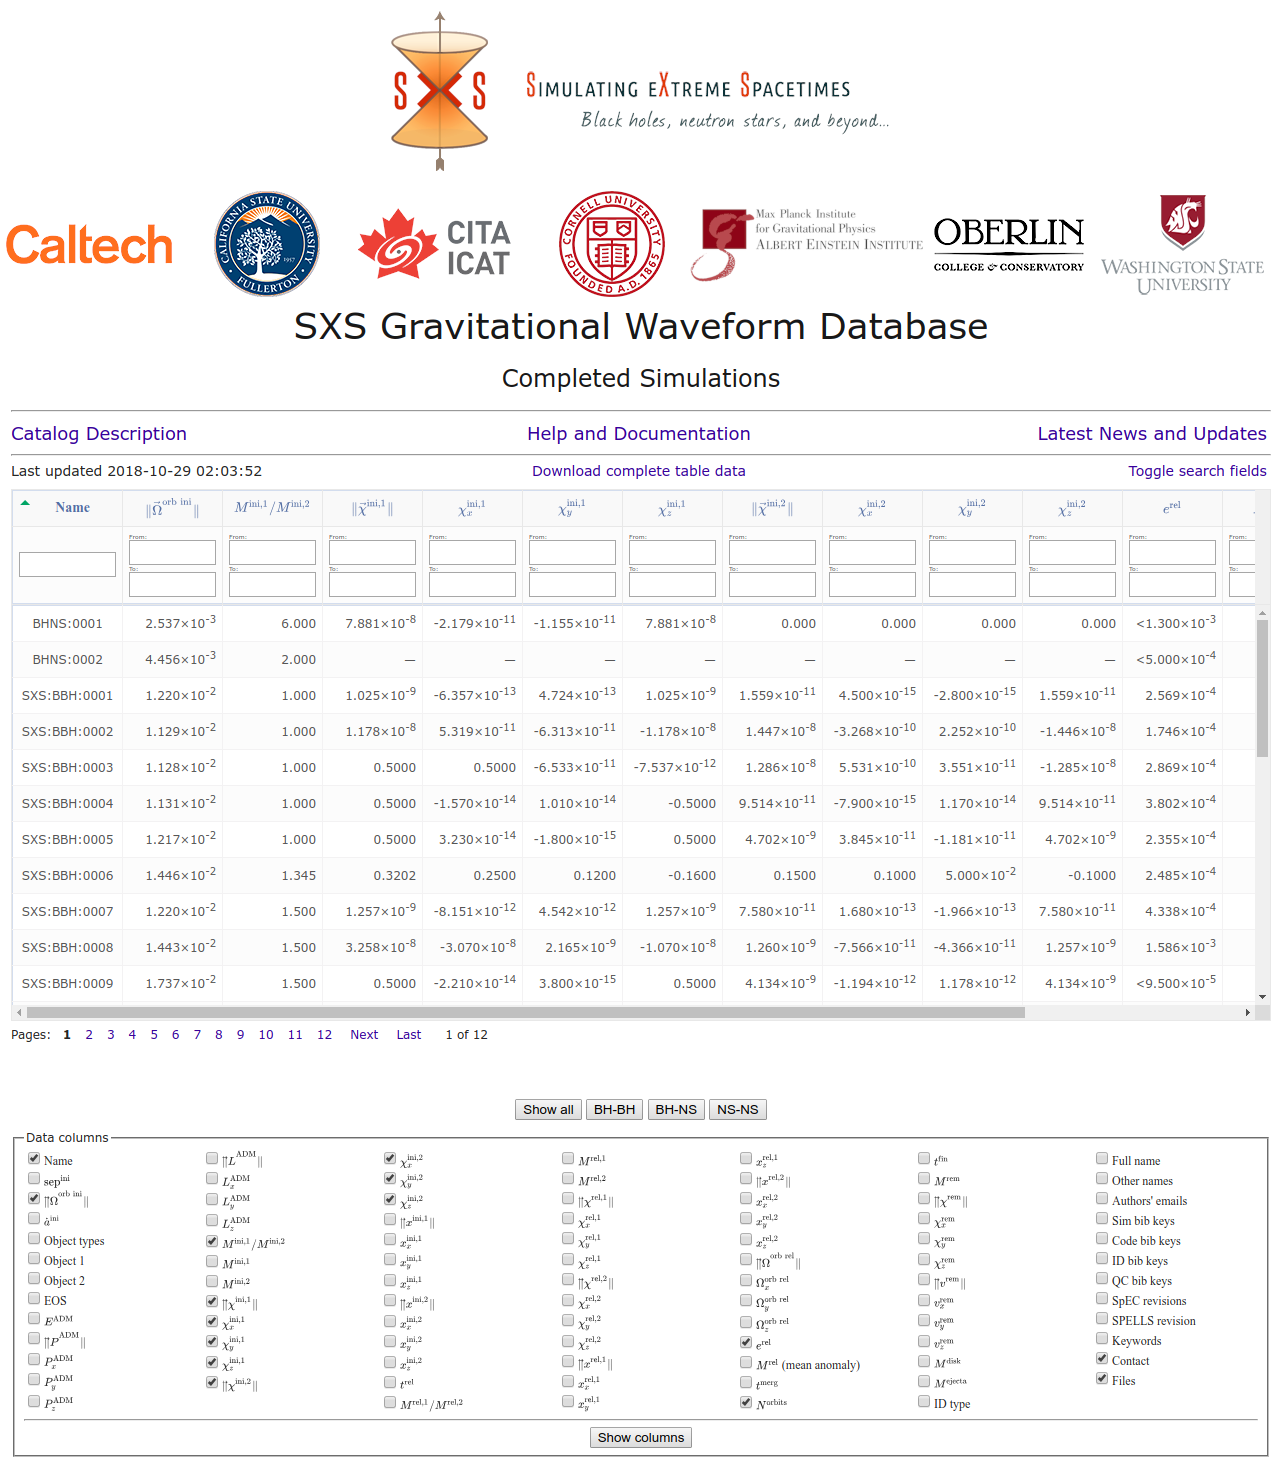
\includegraphics[width=1\textwidth]{figuras/sxs.png}
\caption{Banco de dados de de ondas gravitacionais SXS \href{https://www.black-holes.org/waveforms/catalog.php}{https://www.black-holes.org/waveforms/catalog.php} complementado com as instituições participantes e organizações de financiamento [SXS].}
\label{figsxs}
\end{figure}

A partir desta colaboração entre varias instituições e pesquisadores em 13 de outubro de 2013 um catalogo de simulações de ondas gravitacionais compreendendo 174 formas de onda e que atualmente existem 1377 simulações disponíveis que podem ser baixadas via wget\footnote{\href{https://www.gnu.org/software/wget/}{https://www.gnu.org/software/wget/ (02.12.2018)}} ou diretamente no navegador da web que conta com um litros restringindo os parâmetros (relação de massa, spins, excentricidade, órbitas etc.).

De acordo com a documentação do catalogo as ondas gravitacionais são descartáveis em várias resoluções (variando com o número de simulação individual) e diferentes ordens de extrapolação. Os rótulos de resolução Lev1, Lev2, ... são apenas uma quantidade relativa em uma simulação individual e não são comparáveis entre simulações com parâmetros diferentes. 

A precisão numérica depende da resolução, enquanto a precisão da extrapolação pode ser avaliada pela comparação de diferentes ordens de extrapolação. Pedidos mais altos tendem a produzir melhores resultados no inspiral, mas pior na parte de ringdown \cite{philipp}. 

Desta forma optará por buscar os rótulos de níveis mais elevados nas simulações devido a resultados mais atualizados e mais precisos. Para a facilidade em adquirir os dados será usado um algoritmo automatizado para baixar as simulações via wget, desenvolvido em Python\footnote{\href{https://www.python.org/}{https://www.python.org/ (02.12.2018)}}.

\section{Análise de Dados}
A primeira etapa do processo foi definir quais dados eram importantes e quais poderiam ser utilizados para se obter bons resultados na RNA.

A escolha e adequação dos dados utilizados para treinar e testar uma RNA é de fundamental importância. É necessário que se disponha de dados em quantidade e qualidade suficientes. Caso a quantidade de dados seja pequena, a rede não conseguirá criar um modelo suficientemente representativo para se ter um desempenho satisfatório quando aplicado em situações reais após o seu desenvolvimento, o que é chamado de sobre-ajuste (overfitting) dos dados. Além disto, os dados devem englobar todos os aspectos do problema em questão, a fim de que o modelo
criado seja genérico. Em geral, tais dados precisam ser convertidos para um formato padrão para utilização pelas RNAs. 

Com o objetivo de treinar uma RNA que forneça um diagnóstico classificativo das ondas gravitacionais e que apresente um bom desempenho, os dados colhidos serão tratados, conforme comentado a seguir. 

A descrição do catalogo afirma que dentro de cada simulação tem uma determinada ordem de extrapolação e resolução, a forma de onda é decomposta em harmônicos esféricos ponderados por spin-2 de índices multipolares L de 2 a 8 e M entre +L e −L incluindo 0. Existem imensas diferenças até um fator de \(10^{−7}\) entre determinados modos e o modo dominante (L, M) = (2, 2). Se o fator exceder \(10^{-5}\), os mantenedores do catálogo de ondas gravitacionais recomendam não confiar na precisão do modo específico, porque podem ser tão pequenos que são um ruído puramente numérico.

Portanto, os dados devem ser passados por um tratamento retirando as informações imprecisas das simulações, de modo que, reste somente as informações uteis.

Decerto não será possível usar de todas as simulações advindas do catalogo SXS, dessa forma, inicialmente deverá ser usado somente um grupo de dados destas simulações, para que isto seja possível, ocorrerá o desenvolvimento de um algoritmo que agrupe as simulações com características de spin semelhantes e relação de massas diferentes, a Figura~\ref{figclusterizacao} ilustra como uma porção das simulações esta distribuídas.

\begin{figure}[ht]
\centering
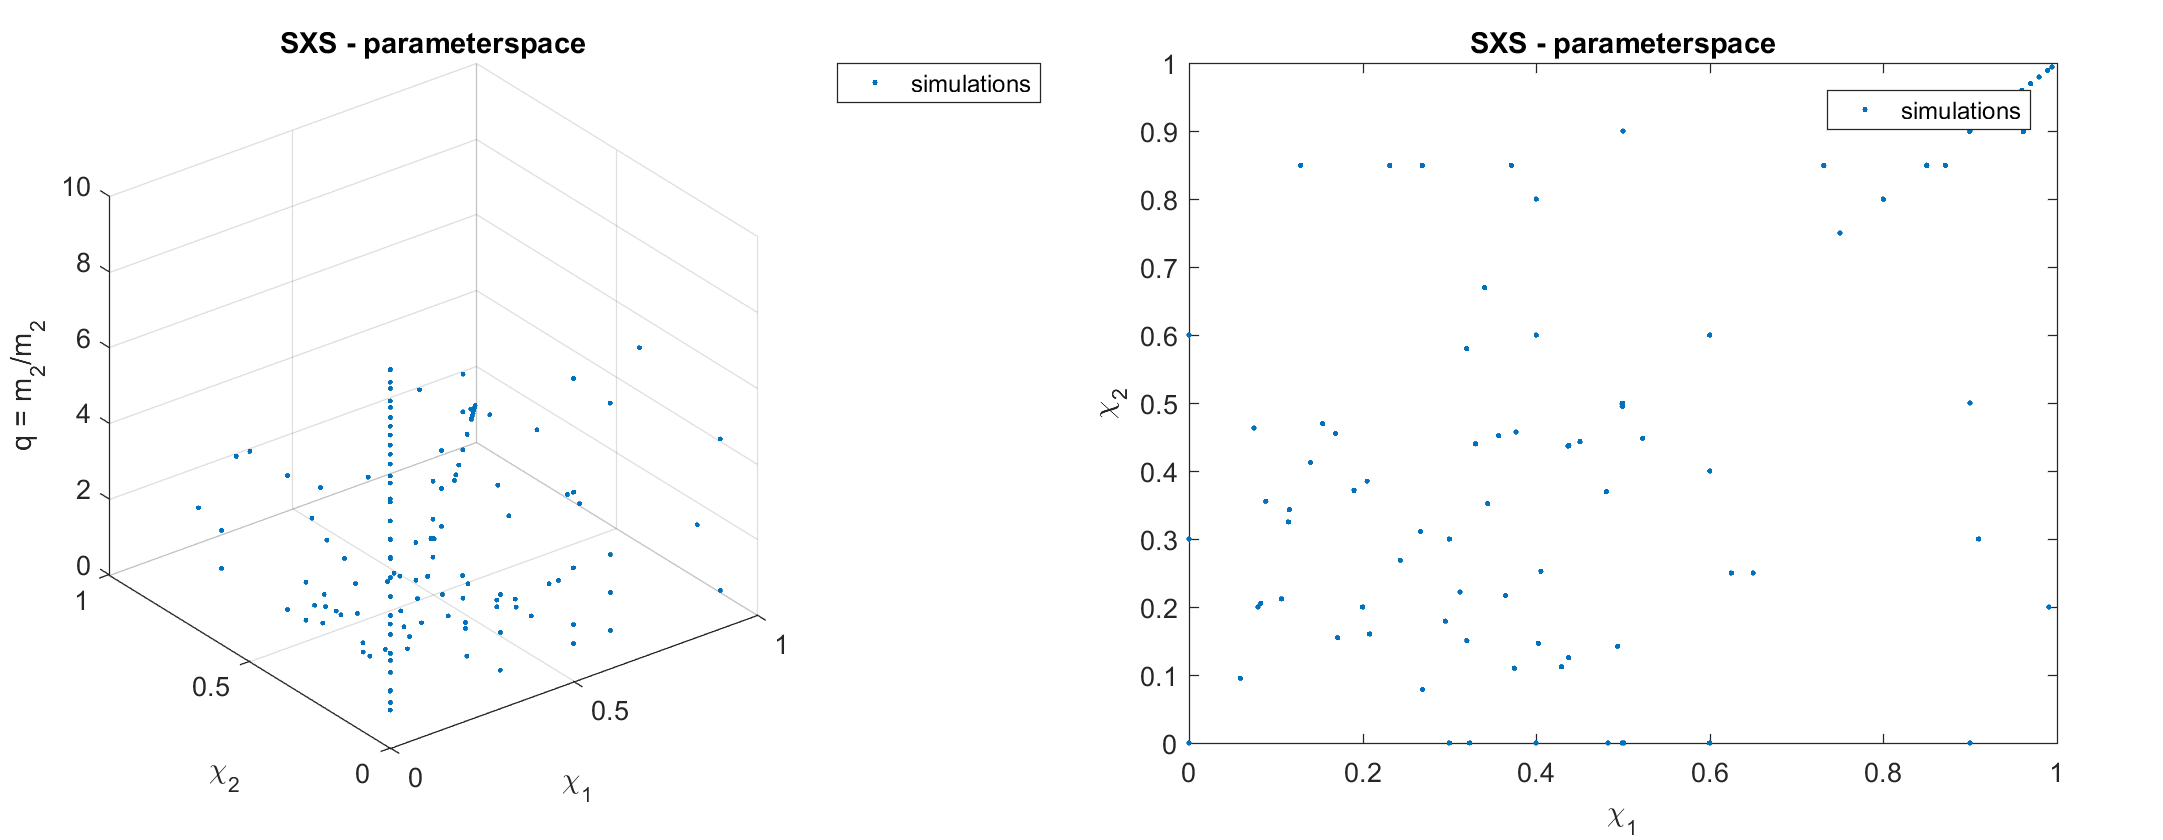
\includegraphics[width=1\textwidth]{figuras/clusterizacao.png}
\caption{Parâmetros do SXS: Dados iniciais em 3D (esquerda) incluindo a taxa de massa \({\nu}\) e 2D (direita) com apenas os spins individuais \(X_1\) e \(X_2\). [Image: \citeonline{philipp}.}
\label{figclusterizacao}
\end{figure}

Em seguida, precisará ser feita a escolha do grupo de simulações com maior quantidade de simulações. em cada simulação existe cerca de 8 arquivos (excluindo os metadados), 6 destes contêm dados de ondas gravitacionais, enquanto 2 descrevem a evolução das órbitas, rotações e outras grandezas geométricas, como a curvatura do espaço-tempo junto com o campo de maré e arrastamento de quadro no Buraco Negro. Com exceção do metadata.txt, os arquivos estão no Formato de Dados Hierárquicos (HDF5) [HDF] com a extensão de arquivo .h5.

Como descrito pelo catalogo, existe comumente dois arquivos com ondas gravitações de maior precisão, são eles,
\textbf{rh\_FiniteRadii\_CodeUnits.h5} e \\
\textbf{rPsi4\_FiniteRadii\_CodeUnits.h5}, esses dois arquivos contêm saída bruta de simulações nas quais as quantidades h e \(\Psi_{4}\) são extraídas em vários raios finitos com grupos h5 rotulados como "Rxxxx.dir", onde "xxxx" é o raio coordenado arredondado para o inteiro mais próximo.

Nas palavras de \cite{philipp}, o arquivo \textbf{rPsi4\_FiniteRadii\_CodeUnits.h5} é o que contem a melhor precisão, dado que representa o melhor estado da arte. Por este motivo o arquivo será usado nesta pesquisa, dentro dele existe varias observações com diferentes esféricos harmônicos, incluindo mais quatro dados que não serão usados nesta pesquisa, por este motivo na analise do arquivo, a Figura~\ref{figpsi4} ilustra o arquivo \textbf{rPsi4\_FiniteRadii\_CodeUnits.h5} aberto em um programa de visualização HDF.

\begin{figure}[ht]
\centering
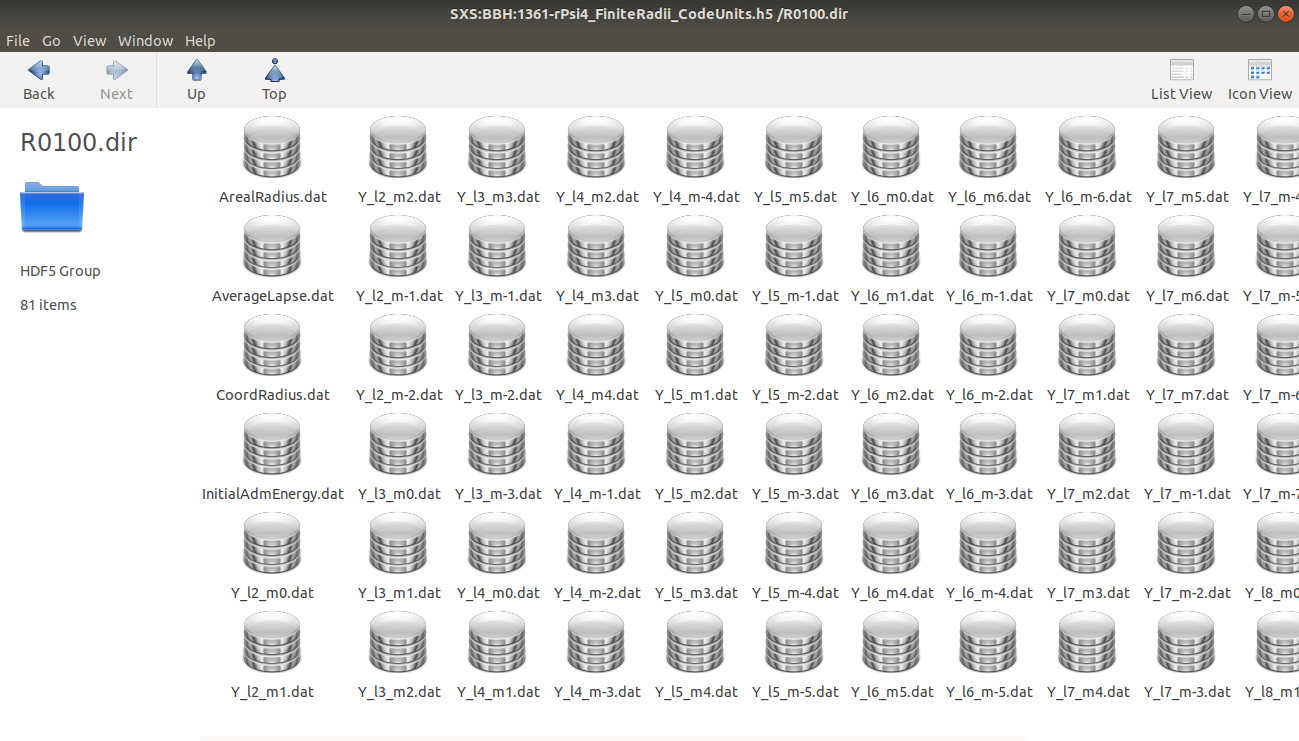
\includegraphics[width=1\textwidth]{figuras/arquivorhpsi4.png}
\caption{Arquivo \textbf{rPsi4\_FiniteRadii\_CodeUnits.h5} aberto com o programa HDFCompass.}
\label{figpsi4}
\end{figure}

Como mencionado anteriormente os harmônicos esféricos ponderados multipolares L e M, quando muito diferentes um do outro podem gerar dados imprecisos, diante disto, necessitará de uma limpeza nos dados a fim de sobrar somente aqueles com os dados que caracterizem  melhor as ondas gravitacionais.

\section{Desenho da pesquisa}
Para a conclusão dos objetivos propostos nesta pesquisa serão realizados algumas etapas as quais visão delinear este trabalho de forma sistemática a fim de garantir o direcionamento da mesma. 

A realização da pesquisa deste trabalho será embasada em experimentos, simulações e análises de dados, seguindo o fluxograma ilustrado na Figura~\ref{figpesquisa}. De forma mais direta, inicialmente a pesquisa constituirá de uma filtragem simplificada dos dados obtidos do grupo SXS, através de técnicas de series temporais afim de trata-los e padronizar os dados para os experimentos. Existem diversas formas de analisar e filtrar dados de series temporais, mais comumente utilizadas como por exemplo os modelos:

\begin{figure}[ht]
\centering
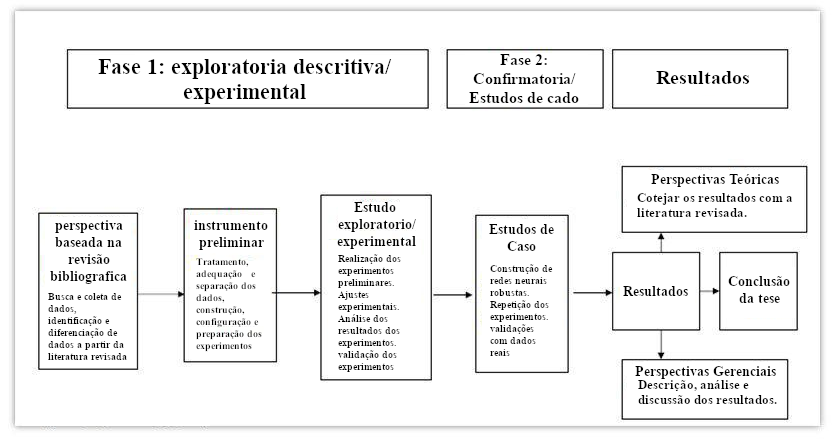
\includegraphics[width=1\textwidth]{figuras/desenho_da_pesquisa.png}
\caption{Desenho da pesquisa}
\label{figpesquisa}
\end{figure}

1 AR(p) → Modelo Auto-Regressivo de Ordem p;

2 MA(q) → Modelo Médias Móveis de Ordem q;

3 ARMA(p, q) → Modelo que combina AR(p) e MA(p);

4 ARIMA(p, d, q) → Modelo ARMA(p, q) com diferenciação de Ordem d.

Sendo que, em primeiro momento, não existirá a necessidade de se utilizar alguma dessas técnicas de analises avançadas, em principio será utilizada somente uma normalização dos dados e uma previa separação de 3 níveis, em que, todas serão padronizadas com a retirada da sua derivada e somadas a uma variação de ruídos uniformes e galicanos que variam entre 10\% e 100\%.

Os níveis gerados após este tratamento de dados serão diferenciados pela janela de informação contida em cada um dos níveis, sendo que, cada um terá um decimo de informação do nível anterior, ilustrado na Figura~\ref{figjanela}, começando com o nível um, o qual, não tem nível anterior e portanto terá uma janela de dados de 8192 pontos, seguido do segundo nível, em que, tem uma janela de informação de 819 pontos e por ultimo o terceiro nível que tem 82 pontos. As janelas de dados possuirão 10\% de sobreposição uma das outras, assim como mostra a Figura~\ref{figjanela}.

\begin{figure}[ht]
\centering
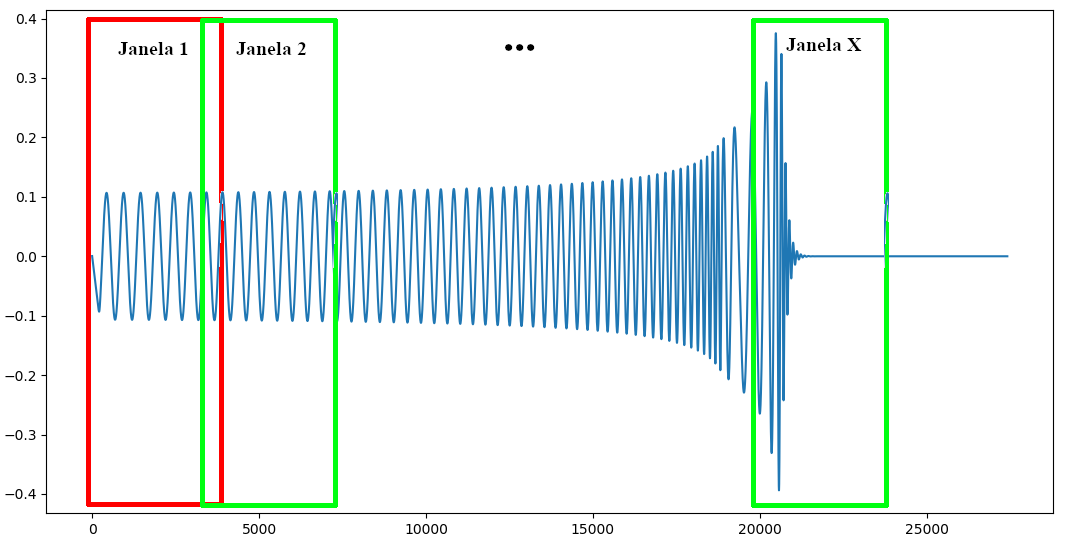
\includegraphics[width=1\textwidth]{figuras/janelas.png}
\caption{Janelas de informação com sobreposição}
\label{figjanela}
\end{figure}

Para obter os resultados e respostas acerca da problematização apresentada neste trabalho, será montado um experimento com redes neurais artificiais do tipo perceptron, mais especificamente do tipo MultiLayerPerceptron, sendo o treinamento realizado através do metodo backpropagation, baseado no método de experimentação dos quadrados latinos, sem a necessidade da analise estatística, conforme é demostrado na Figura~\ref{figexperimento}. No experimento será feita a análise sobre a separabilidade do sinal de informação das ondas gravitacionais e o ruido atrelado a ele, será usado o teste Kolmogorov–Smirnov (também conhecido como teste KS ou teste K–S), o qual, será medido a distancia KS de cada um dos resultados do experimento, ilustrado na Figura~\ref{figkolmogorov}, afim de descobrir o nível de separação das ondas gravitacionais do ruido.

\begin{figure}[ht]
\centering
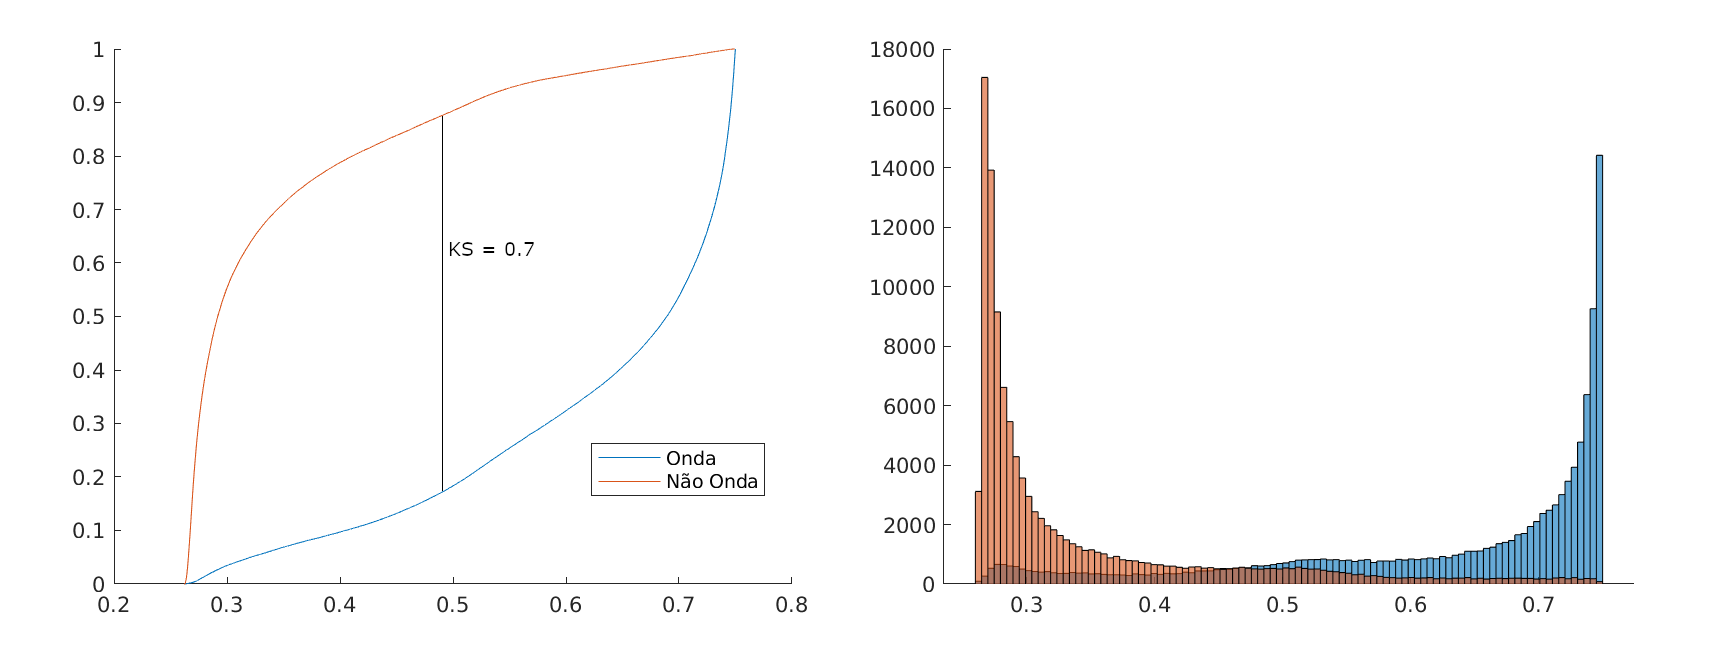
\includegraphics[width=1\textwidth]{figuras/test-kolmogorov.png}
\caption{Gráfico com exemplo do calculo da distancia KS (esquerda) e um Histograma demostrando a separabilidade de classificação.}
\label{figkolmogorov}
\end{figure}

\begin{figure}[ht]
\centering
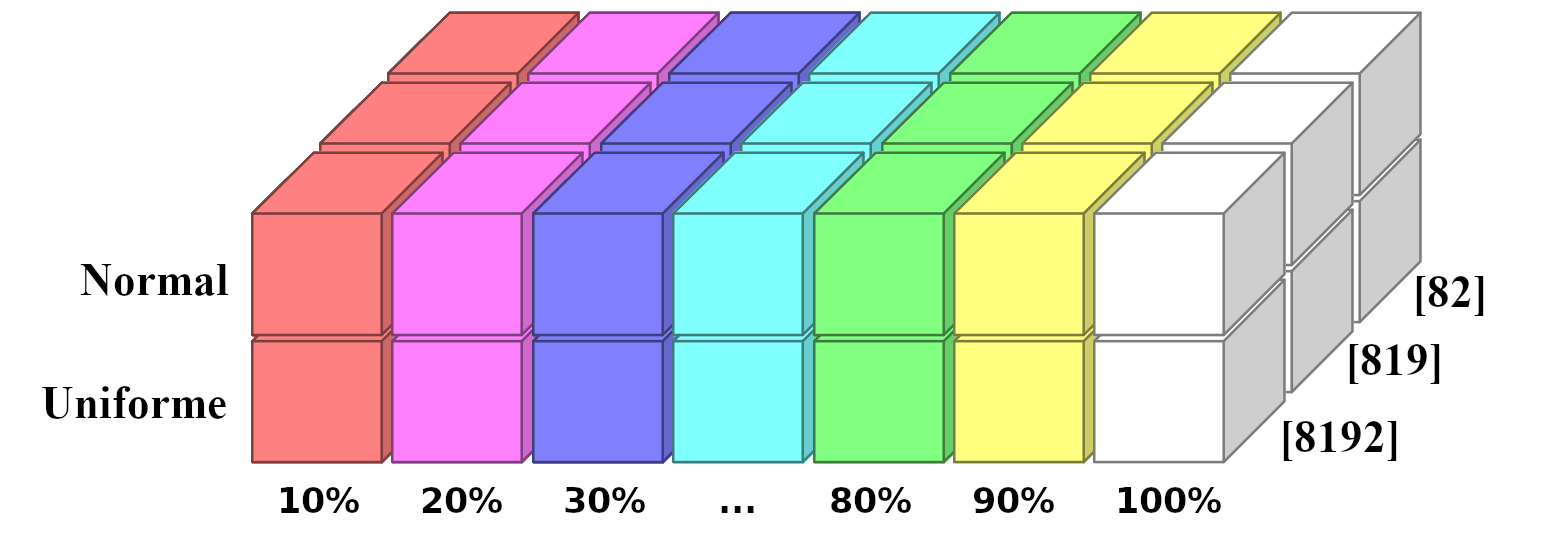
\includegraphics[width=1\textwidth]{figuras/experimento.png}
\caption{Experimento proposto}
\label{figexperimento}
\end{figure}

A rede neural artificial que será usada terá somente duas camadas, sendo, uma de entrada e uma de saída, que contaram com 10 neurônios na primeira camada e 2 neurônios na segunda camada, conforme ilustrado na Figura XX. Como os dados foram separados em 3 níveis, em que, cada um tem uma janela de informações diferente, cada experimento se adequará a este tipo de janela, sendo assim, a rede neural artificial terá uma quantidade de entrada(input) diferente para cada experimento, o qual, mudará o nível da janela de informação.

Após os resultados do primeiro experimento, sucederá uma nova etapa na pesquisa cujo delineamento dar-se-á para testes computacionais com diferentes abordagens de redes neurais artificiais, sendo elas, extreme learnign, Deep e Convulational. seguindo a mesma metodologia da primeira etapa desta pesquisa, desenrolar-se-á, os experimentos feitos anteriormente com abordagens de redes neurais artificiais diferentes para cada experimento, também calculando a distancia de Kolmogorov-Smirnov.

Logo depois de todos os experimentos serem feitos, haverá a necessidade de se fazer uma validação dos experimentos com os dados reais extraídos do LIGO, os quais, serão usados para validação dos experimentos e classificação dos resultados obtidos pelos mesmos.

E finalmente entraremos na etapa final, a qual, será para as analises dos resultados. Nesta analise haverá a necessidade de  se extrair todas as informações possíveis para se alcançar os objetivos desta pesquisa, para começar deverá ser feita uma categorização de todos os KS obtidos através dos experimentos para então classificar a melhor rede e ao mesmo tempo determinar que tipo de ruido existe nos dados reais e em qual amplitude os compõem.

Os resultados obtidos pela analise final serão cotejados com os resultados da literatura revisada. Dado que se os resultados forem satisfatórios, sucederá a descrição, analise e discussão dos resultados, afim de finalizar com a conclusão da escrita da dissertação e a submissão de artigos para revistas e eventos, concluindo assim o mestrado.
\chapter{Cronograma de atividades}
Com o objetivo de detalhar as atividades que comporão a pesquisa e o tempo estimado de implementação, é apresentado o cronograma planejado de execução na Tabela~\ref{tb_cronograma}.

% Please add the following required packages to your document preamble:
% \usepackage{booktabs}
% \usepackage{graphicx}
\begin{table}[h]
\centering
\resizebox{\textwidth}{!}{%
\begin{tabular}{@{}ccccccccccccc@{}}
\toprule
Atividades & Jan. & Fev. & Mar. & Abr. & Maio & Jun. & Jul. & Ago. & Set. & Out. & Nov. & Dez. \\ \midrule
\multicolumn{1}{|l|}{\begin{tabular}[c]{@{}l@{}}Busca e coleta dos dados, identificação e diferenciação \\ dos dados a partir da literatura\end{tabular}} & \multicolumn{1}{c|}{X} & \multicolumn{1}{c|}{X} & \multicolumn{1}{c|}{} & \multicolumn{1}{c|}{} & \multicolumn{1}{c|}{} & \multicolumn{1}{c|}{} & \multicolumn{1}{c|}{} & \multicolumn{1}{c|}{} & \multicolumn{1}{c|}{} & \multicolumn{1}{c|}{} & \multicolumn{1}{c|}{} & \multicolumn{1}{c|}{} \\ \midrule
\multicolumn{1}{|l|}{\begin{tabular}[c]{@{}l@{}}Tratamento, adequação e separação dos dados\\ Construção, configuração e preparação dos experimentos\end{tabular}} & \multicolumn{1}{c|}{} & \multicolumn{1}{c|}{} & \multicolumn{1}{c|}{X} & \multicolumn{1}{c|}{X} & \multicolumn{1}{c|}{} & \multicolumn{1}{c|}{} & \multicolumn{1}{c|}{} & \multicolumn{1}{c|}{} & \multicolumn{1}{c|}{} & \multicolumn{1}{c|}{} & \multicolumn{1}{c|}{} & \multicolumn{1}{c|}{} \\ \midrule
\multicolumn{1}{|l|}{\begin{tabular}[c]{@{}l@{}}Realização dos experimentos preliminares e análise de \\ seus resultados\end{tabular}} & \multicolumn{1}{c|}{} & \multicolumn{1}{c|}{} & \multicolumn{1}{c|}{} & \multicolumn{1}{c|}{} & \multicolumn{1}{c|}{X} & \multicolumn{1}{c|}{X} & \multicolumn{1}{c|}{} & \multicolumn{1}{c|}{} & \multicolumn{1}{c|}{} & \multicolumn{1}{c|}{} & \multicolumn{1}{c|}{} & \multicolumn{1}{c|}{} \\ \midrule
\multicolumn{1}{|l|}{\begin{tabular}[c]{@{}l@{}}Repetição dos experimentos com redes neurais robustas \\ e dados reais\end{tabular}} & \multicolumn{1}{c|}{} & \multicolumn{1}{c|}{} & \multicolumn{1}{c|}{} & \multicolumn{1}{c|}{} & \multicolumn{1}{c|}{} & \multicolumn{1}{c|}{} & \multicolumn{1}{c|}{X} & \multicolumn{1}{c|}{X} & \multicolumn{1}{c|}{} & \multicolumn{1}{c|}{} & \multicolumn{1}{c|}{} & \multicolumn{1}{c|}{} \\ \midrule
\multicolumn{1}{|l|}{\begin{tabular}[c]{@{}l@{}}Descrição, análise, discussão dos resultados e Cotejar os \\ resultados com a literatura revisada\end{tabular}} & \multicolumn{1}{c|}{} & \multicolumn{1}{c|}{} & \multicolumn{1}{c|}{} & \multicolumn{1}{c|}{} & \multicolumn{1}{c|}{} & \multicolumn{1}{c|}{} & \multicolumn{1}{c|}{} & \multicolumn{1}{c|}{} & \multicolumn{1}{c|}{X} & \multicolumn{1}{c|}{} & \multicolumn{1}{c|}{} & \multicolumn{1}{c|}{} \\ \midrule
\multicolumn{1}{|l|}{Escrita dos resultados} & \multicolumn{1}{c|}{} & \multicolumn{1}{c|}{} & \multicolumn{1}{c|}{} & \multicolumn{1}{c|}{} & \multicolumn{1}{c|}{} & \multicolumn{1}{c|}{} & \multicolumn{1}{c|}{} & \multicolumn{1}{c|}{} & \multicolumn{1}{c|}{} & \multicolumn{1}{c|}{X} & \multicolumn{1}{c|}{} & \multicolumn{1}{c|}{} \\ \midrule
\multicolumn{1}{|l|}{Escrita do texto final} & \multicolumn{1}{c|}{} & \multicolumn{1}{c|}{} & \multicolumn{1}{c|}{} & \multicolumn{1}{c|}{} & \multicolumn{1}{c|}{} & \multicolumn{1}{c|}{} & \multicolumn{1}{c|}{} & \multicolumn{1}{c|}{} & \multicolumn{1}{c|}{} & \multicolumn{1}{c|}{} & \multicolumn{1}{c|}{X} & \multicolumn{1}{c|}{} \\ \midrule
\multicolumn{1}{|l|}{Depósito da dissertação} & \multicolumn{1}{c|}{} & \multicolumn{1}{c|}{} & \multicolumn{1}{c|}{} & \multicolumn{1}{c|}{} & \multicolumn{1}{c|}{} & \multicolumn{1}{c|}{} & \multicolumn{1}{c|}{} & \multicolumn{1}{c|}{} & \multicolumn{1}{c|}{} & \multicolumn{1}{c|}{} & \multicolumn{1}{c|}{} & \multicolumn{1}{c|}{X} \\ \midrule
\multicolumn{1}{|l|}{Defesa} & \multicolumn{1}{c|}{} & \multicolumn{1}{c|}{} & \multicolumn{1}{c|}{} & \multicolumn{1}{c|}{} & \multicolumn{1}{c|}{} & \multicolumn{1}{c|}{} & \multicolumn{1}{c|}{} & \multicolumn{1}{c|}{} & \multicolumn{1}{c|}{} & \multicolumn{1}{c|}{} & \multicolumn{1}{c|}{} & \multicolumn{1}{c|}{X} \\ \bottomrule
\end{tabular}%
}
\caption{Cronograma do Mestrado}
\label{tb_cronograma}
\end{table}


% ----------------------------------------------------------
% ELEMENTOS PÓS-TEXTUAIS
% ----------------------------------------------------------
\postextual
% ----------------------------------------------------------

% ----------------------------------------------------------
% Referências bibliográficas
% ----------------------------------------------------------
%\bibliographystyle{IEEEtranN}
\bibliography{referencias.bib}


%---------------------------------------------------------------------
% INDICE REMISSIVO
%---------------------------------------------------------------------
\phantompart
\printindex
%---------------------------------------------------------------------

\end{document}
